\documentclass{article}
\usepackage[utf8]{inputenc}
\usepackage{graphicx}
\usepackage{amsmath}

\title{Intelligens Fejlesztőeszkozok - 4. beadandó}
\author{Sándor Burian}
\date{Szeptember 2022}

\begin{document}

\maketitle

\section{feladat}

Intervallum felező módszerrel 
\begin{equation}
    5x-4 = sin(tanh(-3x+2)); [-10,10] intervallumon 
\end{equation}


\begin{multline}
\\
f(x) = 5x-4-sin(tanh(-3x+2)) \\
a_1 = -10 \\
b_1 = 10\\
f(a_1)=f(-10)=-50-4-sin(tanh(32)) = -54 - 0,017452406 = -54,017452406 \\
f(b_1)=f(10) = 50-4 - sin(tanh(-28)) = 46 - (-0,017452406) = 46,017452406 \\
\\
\Rightarrow f(a)f(b)<0 \Rightarrow intervallumfelezes: \dfrac{a+b}{2} \Rightarrow \frac{10+(-10)}{2} = 0 \\
\end{multline}

\begin{multline}
\\
f(0) = -4-sin(tanh(2)) = -4-0,016824661 = -4,016824661\\
a_2 = (a_1 + b_1)/2 = 0; f(a_2) < 0
b_2 = b_1=10\\
f(b_2) >0\\
f(\dfrac{a_2+b_2}{2}) = f(5) = 25-4-sin(tanh(-13)) = 21,017452406 \\
b_3 = 5\\
f(b_3) > 0 \\
a_3 = a_2 = 0 \\
f(a_3)<0\\
f(0)f(5) < 0 \\
f(2.5) = 12.5-4-sin=tanh(-5.5)) = 8,517451824 \\
...\\
f(\dfrac{a_23 + b_23}{2}) = f(0,798685552) = 0,000000094 \\
\Rightarrow x = 0,798685552\\
\end{multline}

Julia kódként:

\begin{verbatim}
f(x)=5*x-4-sin(tanh(-3*x+2))
a=-10
b=10
ϵ=1e-7 #(10^(-7))

while true
    global a,b
    c=(a+b)/2
    println("x= ",c)
    println("f(x)= ",f(c))
    println()
    if sign(f(c))==sign(f(a))
        a=c
    end
    if sign(f(c))==sign(f(b))
        b=c
    end
    if abs(f(c))<ϵ
        break
    end
end
\end{verbatim}

Logok:

\begin{verbatim}
x= 0.0  
f(x)= -4.821494815516438

x= 5.0
f(x)= 21.841470984802374

x= 2.5
f(x)= 9.341452936704993

x= 1.25
f(x)= 3.0583686122902405

x= 0.625
f(x)= -0.9990327572022525

x= 0.9375
f(x)= 1.3092437102511458

x= 0.78125
f(x)= 0.2310697309851627

x= 0.703125
f(x)= -0.37564942969465204

x= 0.7421875
f(x)= -0.06813638549908974

x= 0.76171875
f(x)= 0.08270992936515631

x= 0.751953125
f(x)= 0.007575155275291817

x= 0.7470703125
f(x)= -0.030211616196670926

x= 0.74951171875
f(x)= -0.011300580891388218

x= 0.750732421875
f(x)= -0.001858251535921368

x= 0.7513427734375
f(x)= 0.0028595732281952724

x= 0.75103759765625
f(x)= 0.0005009404338206236

x= 0.750885009765625
f(x)= -0.0006785857483954938

x= 0.7509613037109375
f(x)= -8.880519482826199e-5

x= 0.7509994506835938
f(x)= 0.0002060719865843441

x= 0.7509803771972656
f(x)= 5.863448746595834e-5

x= 0.7509708404541016
f(x)= -1.5085080807220042e-5

x= 0.7509756088256836
f(x)= 2.1774771550742145e-5

x= 0.7509732246398926
f(x)= 3.3448624267573557e-6

x= 0.7509720325469971
f(x)= -5.8701049265030836e-6

x= 0.7509726285934448
f(x)= -1.2626201839338602e-6

x= 0.7509729266166687
f(x)= 1.0411213878791514e-6

x= 0.7509727776050568
f(x)= -1.107493314278507e-7

x= 0.7509728521108627
f(x)= 4.6518604487899573e-7

x= 0.7509728148579597
f(x)= 1.7721836090278664e-7

x= 0.7509727962315083
f(x)= 3.323451580605763e-8
\end{verbatim}

Ábrázolva:

\includegraphics[scale=1]{../plot_2.png} 

\section{feladat}

\begin{equation}
x+3= e^{sin(x+3)}
\end{equation}

Intervallum felező módszerrel [-10,10] között.

Matematikai levezetés hasonlatos.

Julia kód:

\begin{verbatim}
f(x)=x+3-ℯ^(sin(x+3))
a=-10
b=10
ϵ=1e-7 #(10^(-7))

while true
    global a,b
    c=(a+b)/2
    println("x= ",c)
    println("f(x)= ",f(c))
    println()
    if sign(f(c))==sign(f(a))
        a=c
    end
    if sign(f(c))==sign(f(b))
        b=c
    end
    if abs(f(c))<ϵ
        break
    end
end
\end{verbatim}

Logok:

\begin{verbatim}
x= 0.0  
f(x)= 1.848437163485465

x= -5.0
f(x)= -2.402807126123528 

x= -2.5
f(x)= -1.1151462964420837

x= -1.25
f(x)= -0.9250978172453692

x= -0.625
f(x)= 0.3739240078773549 

x= -0.9375
f(x)= -0.35209068903115126  

x= -0.78125
f(x)= -0.0008356627438894648

x= -0.703125
f(x)= 0.18456173681073818   

x= -0.7421875
f(x)= 0.0912498148899128

x= -0.76171875
f(x)= 0.04503881542828969

x= -0.771484375
f(x)= 0.022057630510200266

x= -0.7763671875
f(x)= 0.010599761786235007

x= -0.77880859375
f(x)= 0.004879214512186092

x= -0.780029296875
f(x)= 0.0020210634445905207

x= -0.7806396484375
f(x)= 0.0005925217794442439

x= -0.78094482421875
f(x)= -0.00012161518258224646

x= -0.780792236328125
f(x)= 0.00023544213054549346

x= -0.7808685302734375
f(x)= 5.691068110946773e-5

x= -0.7809066772460938
f(x)= -3.23529490668939e-5

x= -0.7808876037597656
f(x)= 1.2278691452927148e-5

x= -0.7808971405029297
f(x)= -1.0037172450960696e-5

x= -0.7808923721313477
f(x)= 1.1207485899333847e-6

x= -0.7808947563171387
f(x)= -4.458214657887538e-6

x= -0.7808935642242432
f(x)= -1.668733716098103e-6

x= -0.7808929681777954
f(x)= -2.739927333905712e-7

x= -0.7808926701545715
f(x)= 4.233778856388426e-7

x= -0.7808928191661835
f(x)= 7.469256546599468e-8
\end{verbatim}

Ábrázolva:

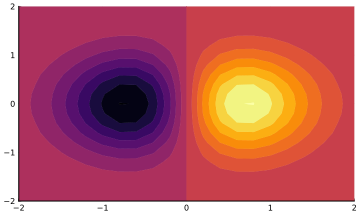
\includegraphics[scale=1]{../plot_3.png} 

\section{feladat}

\begin{equation}
6x+3 = tanh(tan(cos(-4x^{2}-3)))
\end{equation}

[-10,10] tartományon, Húr módszerrel

Húr engyelete:
\begin{multline}
a_0 = -10\\
x_0 = 10\\
f(-10)=-60+3-tanh(tan(cos(-403))) = -57.01276453\\
f(10) = 60+3-tanh(tan(cos(-403))) = 62.98723547\\
\end{multline}

innen 
\begin{multline}
x_{n+1} = a - \dfrac{x_n - a}{f(x_n) - f(a)} \dot{•} f(a)\\
f(x_n) \lt \epsilon \Rightarrow leall \Rightarrow x_n
\end{multline}

Julia kód:

\begin{verbatim}
f(x)=6*x+3-tanh(tan(cos(-4*x^2-3)))
a=-10
x=10
ϵ=1e-7

while true
    global x
    x=a-f(a)*(x-a)/(f(x)-f(a))
    println("x= ",x)
    println("f(x)= ",f(x))
    println()
    if abs(f(x))<ϵ
        break
    end
end
\end{verbatim}

logok

\begin{verbatim}
x= -0.3946673776396814
f(x)= 1.473222596433957

x= -0.6340843608639908    
f(x)= -0.7005580211701712 

x= -0.518834024842656     
f(x)= 0.475196224620007   

x= -0.5963702836862499    
f(x)= -0.29263090201165215

x= -0.5483789490399076    
f(x)= 0.19549112038083016 

x= -0.5803310204365939    
f(x)= -0.1252049477592092 

x= -0.5598223266568301
f(x)= 0.08271525237683225

x= -0.5733517486254289
f(x)= -0.05364104222537219

x= -0.564569711701985
f(x)= 0.035233678627016984

x= -0.5703345962277488
f(x)= -0.022957362273294757

x= -0.5665768482960285
f(x)= 0.015039215196470612

x= -0.5690378817376001
f(x)= -0.009817990684844624

x= -0.5674309813764502
f(x)= 0.006424128784621008

x= -0.5684822946895061
f(x)= -0.004197205014267735

x= -0.5677953690318347
f(x)= 0.002744922160006602

x= -0.568244588846385
f(x)= -0.001794004529417248

x= -0.5679509821710642
f(x)= 0.0011730000376027339

x= -0.5681429513807323
f(x)= -0.0007667509786616344

x= -0.5680174658453687
f(x)= 0.0005012887629938789

x= -0.5680995054428433
f(x)= -0.0003276959548840219

x= -0.5680458752817863
f(x)= 0.0002142334239423893

x= -0.5680809362282222
f(x)= -0.00014004957144803099

x= -0.5680580159837305
f(x)= 9.15567689105945e-5

x= -0.5680729999652794
f(x)= -5.98535484045426e-5

x= -0.5680632044536296
f(x)= 3.912869655703366e-5

x= -0.568069608173257
f(x)= -2.557978649297965e-5

x= -0.5680654218377033
f(x)= 1.6722493205334477e-5

x= -0.5680681586059535
f(x)= -1.0932096461913066e-5

x= -0.5680663694815777
f(x)= 7.146723589424031e-6

x= -0.5680675390994843
f(x)= -4.672074870593068e-6

x= -0.5680667744773746
f(x)= 3.054309705152747e-6

x= -0.5680672743393593
f(x)= -1.9967148497945786e-6

x= -0.5680669475611424
f(x)= 1.3053267006735148e-6

x= -0.5680671611882016
f(x)= -8.533403115240645e-7

x= -0.5680670215322934
f(x)= 5.57860228067586e-7

x= -0.5680671128305423
f(x)= -3.6469388708937345e-7

x= -0.5680670531454961
f(x)= 2.3841391838530512e-7

x= -0.5680670921638242
f(x)= -1.5586001317346998e-7

x= -0.5680670666560967
f(x)= 1.0189147403583121e-7

x= -0.5680670833314441
f(x)= -6.66102302204763e-8
\end{verbatim}

árbrázolva:

\includegraphics[scale=1]{../plot_4.png} 

\section{feladat}
\begin{equation}
x+2 = x^{3}
\end{equation}

[-10,10] tartományon, Newton-Raphson módszerrel

\begin{multline}
x_{n+1} = \frac{f(x_n)}{f'(x_n)} \\
\end{multline}

ahol jelen esetben

\begin{multline}
\\
f(x) = x+2 - x^{3}\\
f'(x) = 1-3x^{2}\\
f"(x) = -6x\\
\\
f(-10) = -8+1000= 992\\
f'(-10) = 1 - 300 = -299\\
f"(-10) = 60\\
f(10) = 12-1000 = -988\\
\end{multline}

alapján 

\begin{multline}
\\
sign(f(-10)) = 1\\
sign(f'(-10)) = -1\\
sign(f"(-10)) = 1\\
sign(f(10)) = -1\\
\end{multline}

Mivel \textit{f'(-10)} és \textit{f(-10)} valamint \textit{f"(-10)} és \textit{f(10)} előjelei megegyeznek ezért helyes intervallumon vagyunk, a művelet elvégezhető.


Julia kód:

\begin{verbatim}
f(x)=x+2-x^3
df(x)=1-3*x^2

x=-10
ϵ=1e-7

while true
    global x
    x=x-f(x)/df(x)
    println("x= ",x)
    println("f(x)= ",f(x))
    println()
    if abs(f(x))<ϵ
        break
    end
end
\end{verbatim}

Logok:

\begin{verbatim}
x= -6.682274247491639  
f(x)= 293.6999085590051

x= -4.473312792869828   
f(x)= 87.04003516198537 

x= -2.9988472242547655  
f(x)= 25.970039789119255

x= -1.999201900879969   
f(x)= 7.991224730944533 

x= -1.2720939925431056  
f(x)= 2.7864379244631436

x= -0.5492206014655907  
f(x)= 1.6164480962034022

x= -17.551900926196666  
f(x)= 5391.648634395187 

x= -11.711775501850084  
f(x)= 1596.741938527522 

x= -7.821998670703618
f(x)= 472.75653358358846

x= -5.232275467424355
f(x)= 140.01019468202122

x= -3.506526815777292
f(x)= 41.608781234980135

x= -2.3470941558915683
f(x)= 12.58269777701162

x= -1.5366954902088426
f(x)= 4.092107996851008

x= -0.864126976223906
f(x)= 1.7811299712985802

x= 0.572098718429206
f(x)= 2.3848525564336365

x= -131.12099781689727
f(x)= 2.2541969650863465e6

x= -87.4156545880499
f(x)= 667901.0175286231

x= -58.27955805586903
f(x)= 197890.64076094175

x= -38.8566558177144
f(x)= 58630.4649589283

x= -25.909715855150342
f(x)= 17369.62909815448

x= -17.280731383904506
f(x)= 5145.154818537878

x= -11.53112653863139
f(x)= 1523.7267835392222

x= -7.701711255066577
f(x)= 451.13573733453586

x= -5.152188160809331
f(x)= 133.61286731020152

x= -3.4530383049803026
f(x)= 39.71917254207688

x= -2.3107118145696806
f(x)= 12.027077638259073

x= -1.5098765713570435
f(x)= 3.9322302087075345

x= -0.8364551305833876
f(x)= 1.7487767118602822

x= 0.7548296498241522
f(x)= 2.3247520206776104

x= 4.032343923946572
f(x)= -59.5327518144143

x= 2.7863516954778125
f(x)= -16.84620236002299

x= 2.030620667549976
f(x)= -4.342481805448995

x= 1.6487049095196127
f(x)= -0.8328507392434155

x= 1.5322985411023986
f(x)= -0.06544468594788322

x= 1.5214701702523892
f(x)= -0.0005377329652014318

x= 1.5213797130880249
f(x)= -3.734754283613029e-8
\end{verbatim}

Mivel az utolsó kapott érték az intervallumon belül van így elfogadjuk.


\section{feladat}
\begin{equation}
f(x)= sin(x-5)
\end{equation}

[-10,10] tartományon, Fixpont iterációval kiindulópont x_0 = 5,5

\begin{multline}
\\
f(x)=0\\
sin(x-5)=0\\
\\
g(x) = sin(x-5)\\
\end{multline}

\begin{multline}
x_0 = 5.5
x_1 = g(x_0) = sin(0.5) = 0.479425538604203
x_2 = g(x_1) = sin(0.479425538604203-5) = 0.981659930640367
x_3 = g(x_2) = sin(0.981659930640367-5) = 0.768662417852264
\end{multline}

Julia kód:

\begin{verbatim}
g(x)=sin(x-5)
x=5.5

ϵ=1e-7

while true
    global x
    x=g(x)
    println("x= ",x)
    println("g(x)= ",g(x))
    println("f(x)= ",sin(x-5))
    if abs(x-g(x))<ϵ
        break
    end
end
\end{verbatim}

logok:

\begin{verbatim}
x= 0.479425538604203    
g(x)= 0.9816599306403665
f(x)= 0.9816599306403665
x= 0.9816599306403665   
g(x)= 0.768662417852264 
f(x)= 0.768662417852264 
x= 0.768662417852264    
g(x)= 0.8865089187986952
f(x)= 0.8865089187986952
x= 0.8865089187986952   
g(x)= 0.8259574064776428
f(x)= 0.8259574064776428
x= 0.8259574064776428
g(x)= 0.858557690332052
f(x)= 0.858557690332052
x= 0.858557690332052
g(x)= 0.8413897441305478
f(x)= 0.8413897441305478
x= 0.8413897441305478
g(x)= 0.8505433492252111
f(x)= 0.8505433492252111
x= 0.8505433492252111
g(x)= 0.8456938576460371
f(x)= 0.8456938576460371
x= 0.8456938576460371
g(x)= 0.8482719233199884
f(x)= 0.8482719233199884
x= 0.8482719233199884
g(x)= 0.84690386307505
f(x)= 0.84690386307505
x= 0.84690386307505
g(x)= 0.8476305309324842
f(x)= 0.8476305309324842
x= 0.8476305309324842
g(x)= 0.8472447467097592
f(x)= 0.8472447467097592
x= 0.8472447467097592
g(x)= 0.8474496132890567
f(x)= 0.8474496132890567
x= 0.8474496132890567
g(x)= 0.8473408367894607
f(x)= 0.8473408367894607
x= 0.8473408367894607
g(x)= 0.8473985974753907
f(x)= 0.8473985974753907
x= 0.8473985974753907
g(x)= 0.8473679276060092
f(x)= 0.8473679276060092
x= 0.8473679276060092
g(x)= 0.8473842130985798
f(x)= 0.8473842130985798
x= 0.8473842130985798
g(x)= 0.847375565711761
f(x)= 0.847375565711761
x= 0.847375565711761
g(x)= 0.8473801573907789
f(x)= 0.8473801573907789
x= 0.8473801573907789
g(x)= 0.847377719261386
f(x)= 0.847377719261386
x= 0.847377719261386
g(x)= 0.8473790138826188
f(x)= 0.8473790138826188
x= 0.8473790138826188
g(x)= 0.8473783264528985
f(x)= 0.8473783264528985
x= 0.8473783264528985
g(x)= 0.8473786914707411
f(x)= 0.8473786914707411
x= 0.8473786914707411
g(x)= 0.8473784976502133
f(x)= 0.8473784976502133
x= 0.8473784976502133
g(x)= 0.847378600566832
f(x)= 0.847378600566832
x= 0.847378600566832
g(x)= 0.8473785459192169
f(x)= 0.8473785459192169
\end{verbatim}

Ábrázolva:

\includegraphics[scale=1]{../plot_8_1.png} 

\section{feladat}
\begin{equation}
f(x)= cos(x-6) =0
\end{equation}
hasonlóan, kiindulópont x_0 = 2; 

\begin{multline}
x_0 = 2
x_1 = g(x_0) = cos(-4) = -0.653643620863612\\
x_2 = g(x_1) = cos(-0.653643620863612-6) = 0.932161514392666\\
x_3 = g(x_2) = cos(0.932161514392666-6) = 0.348011807099133\\
...\\
\end{multline}

Julia kód:

\begin{verbatim}
#fixpont iteráció
#f(x)=cos(x-5)
#x=g(x)

g(x)= cos(x-5)

x=2
ϵ=1e-7

while true
    global x
    x=g(x)
    println("x= ",x)
    println("g(x)= ",g(x))
    println("f(x)= ",cos(x-5))
    if abs(x-g(x))<ϵ
        break
    end
end
\end{verbatim}

logok:

\begin{verbatim}
f(x)= 0.1435582818229001
x= 0.1435582818229001
g(x)= 0.14355504347494927
f(x)= 0.14355504347494927
x= 0.14355504347494927
g(x)= 0.14355824828042116
f(x)= 0.14355824828042116
x= 0.14355824828042116
g(x)= 0.14355507667000642
f(x)= 0.14355507667000642
x= 0.14355507667000642
g(x)= 0.14355821542920247
f(x)= 0.14355821542920247
x= 0.14355821542920247
g(x)= 0.14355510918096287
f(x)= 0.14355510918096287
x= 0.14355510918096287
g(x)= 0.1435581832549984
f(x)= 0.1435581832549984
x= 0.1435581832549984
g(x)= 0.14355514102191658
f(x)= 0.14355514102191658
x= 0.14355514102191658
g(x)= 0.1435581517438569
f(x)= 0.1435581517438569
x= 0.1435581517438569
g(x)= 0.14355517220667544
f(x)= 0.14355517220667544
x= 0.14355517220667544
g(x)= 0.14355812088211342
f(x)= 0.14355812088211342
x= 0.14355812088211342
g(x)= 0.14355520274876254
f(x)= 0.14355520274876254
x= 0.14355520274876254
g(x)= 0.14355809065638464
f(x)= 0.14355809065638464
x= 0.14355809065638464
g(x)= 0.14355523266142325
f(x)= 0.14355523266142325
x= 0.14355523266142325
g(x)= 0.14355806105356236
f(x)= 0.14355806105356236
x= 0.14355806105356236
g(x)= 0.14355526195762777
f(x)= 0.14355526195762777
x= 0.14355526195762777
g(x)= 0.14355803206081083
f(x)= 0.14355803206081083
x= 0.14355803206081083
g(x)= 0.14355529065008177
f(x)= 0.14355529065008177
x= 0.14355529065008177
g(x)= 0.14355800366555632
f(x)= 0.14355800366555632
x= 0.14355800366555632
g(x)= 0.14355531875122626
f(x)= 0.14355531875122626
x= 0.14355531875122626
g(x)= 0.14355797585548608
f(x)= 0.14355797585548608
x= 0.14355797585548608
g(x)= 0.14355534627324837
f(x)= 0.14355534627324837
x= 0.14355534627324837
g(x)= 0.14355794861853963
f(x)= 0.14355794861853963
x= 0.14355794861853963
g(x)= 0.14355537322808198
f(x)= 0.14355537322808198
x= 0.14355537322808198
g(x)= 0.1435579219429062
f(x)= 0.1435579219429062
x= 0.1435579219429062
g(x)= 0.14355539962741662
f(x)= 0.14355539962741662
x= 0.14355539962741662
g(x)= 0.14355789581701836
f(x)= 0.14355789581701836
x= 0.14355789581701836
g(x)= 0.14355542548270012
f(x)= 0.14355542548270012
x= 0.14355542548270012
g(x)= 0.14355787022954616
f(x)= 0.14355787022954616
x= 0.14355787022954616
g(x)= 0.14355545080514387
f(x)= 0.14355545080514387
x= 0.14355545080514387
g(x)= 0.1435578451693942
f(x)= 0.1435578451693942
x= 0.1435578451693942
g(x)= 0.14355547560572982
f(x)= 0.14355547560572982
x= 0.14355547560572982
g(x)= 0.14355782062569397
f(x)= 0.14355782062569397
x= 0.14355782062569397
g(x)= 0.1435554998952132
f(x)= 0.1435554998952132
x= 0.1435554998952132
g(x)= 0.14355779658780274
f(x)= 0.14355779658780274
x= 0.14355779658780274
g(x)= 0.1435555236841268
f(x)= 0.1435555236841268
x= 0.1435555236841268
g(x)= 0.14355777304529674
f(x)= 0.14355777304529674
x= 0.14355777304529674
g(x)= 0.14355554698278544
f(x)= 0.14355554698278544
x= 0.14355554698278544
g(x)= 0.14355774998796667
f(x)= 0.14355774998796667
x= 0.14355774998796667
g(x)= 0.14355556980129386
f(x)= 0.14355556980129386
x= 0.14355556980129386
g(x)= 0.1435577274058132
f(x)= 0.1435577274058132
x= 0.1435577274058132
g(x)= 0.14355559214954672
f(x)= 0.14355559214954672
x= 0.14355559214954672
g(x)= 0.14355770528904546
f(x)= 0.14355770528904546
x= 0.14355770528904546
g(x)= 0.14355561403723482
f(x)= 0.14355561403723482
x= 0.14355561403723482
g(x)= 0.14355768362807114
f(x)= 0.14355768362807114
x= 0.14355768362807114
g(x)= 0.1435556354738502
f(x)= 0.1435556354738502
x= 0.1435556354738502
g(x)= 0.14355766241349657
f(x)= 0.14355766241349657
x= 0.14355766241349657
g(x)= 0.14355565646868898
f(x)= 0.14355565646868898
x= 0.14355565646868898
g(x)= 0.1435576416361233
f(x)= 0.1435576416361233
x= 0.1435576416361233
g(x)= 0.1435556770308556
f(x)= 0.1435556770308556
x= 0.1435556770308556
g(x)= 0.14355762128694088
f(x)= 0.14355762128694088
x= 0.14355762128694088
g(x)= 0.14355569716926644
f(x)= 0.14355569716926644
x= 0.14355569716926644
g(x)= 0.14355760135712436
f(x)= 0.14355760135712436
x= 0.14355760135712436
g(x)= 0.14355571689265417
f(x)= 0.14355571689265417
x= 0.14355571689265417
g(x)= 0.14355758183803255
f(x)= 0.14355758183803255
x= 0.14355758183803255
g(x)= 0.14355573620957213
f(x)= 0.14355573620957213
x= 0.14355573620957213
g(x)= 0.1435575627211991
f(x)= 0.1435575627211991
x= 0.1435575627211991
g(x)= 0.14355575512839786
f(x)= 0.14355575512839786
x= 0.14355575512839786
g(x)= 0.14355754399833523
f(x)= 0.14355754399833523
x= 0.14355754399833523
g(x)= 0.143555773657334
f(x)= 0.143555773657334
x= 0.143555773657334
g(x)= 0.14355752566132274
f(x)= 0.14355752566132274
x= 0.14355752566132274
g(x)= 0.1435557918044162
f(x)= 0.1435557918044162
x= 0.1435557918044162
g(x)= 0.1435575077022086
f(x)= 0.1435575077022086
x= 0.1435575077022086
g(x)= 0.1435558095775139
f(x)= 0.1435558095775139
x= 0.1435558095775139
g(x)= 0.14355749011320507
f(x)= 0.14355749011320507
x= 0.14355749011320507
g(x)= 0.14355582698433492
f(x)= 0.14355582698433492
x= 0.14355582698433492
g(x)= 0.14355747288668352
f(x)= 0.14355747288668352
x= 0.14355747288668352
g(x)= 0.14355584403242705
f(x)= 0.14355584403242705
x= 0.14355584403242705
g(x)= 0.1435574560151761
f(x)= 0.1435574560151761
x= 0.1435574560151761
g(x)= 0.1435558607291834
f(x)= 0.1435558607291834
x= 0.1435558607291834
g(x)= 0.14355743949136537
f(x)= 0.14355743949136537
x= 0.14355743949136537
g(x)= 0.14355587708184406
f(x)= 0.14355587708184406
x= 0.14355587708184406
g(x)= 0.14355742330808588
f(x)= 0.14355742330808588
x= 0.14355742330808588
g(x)= 0.1435558930975007
f(x)= 0.1435558930975007
x= 0.1435558930975007
g(x)= 0.14355740745831896
f(x)= 0.14355740745831896
x= 0.14355740745831896
g(x)= 0.14355590878309896
f(x)= 0.14355590878309896
x= 0.14355590878309896
g(x)= 0.1435573919351928
f(x)= 0.1435573919351928
x= 0.1435573919351928
g(x)= 0.14355592414543952
f(x)= 0.14355592414543952
x= 0.14355592414543952
g(x)= 0.14355737673197527
f(x)= 0.14355737673197527
x= 0.14355737673197527
g(x)= 0.14355593919118595
f(x)= 0.14355593919118595
x= 0.14355593919118595
g(x)= 0.1435573618420723
f(x)= 0.1435573618420723
x= 0.1435573618420723
g(x)= 0.14355595392686202
f(x)= 0.14355595392686202
x= 0.14355595392686202
g(x)= 0.14355734725902866
f(x)= 0.14355734725902866
x= 0.14355734725902866
g(x)= 0.143555968358857
f(x)= 0.143555968358857
x= 0.143555968358857
g(x)= 0.1435573329765201
f(x)= 0.1435573329765201
x= 0.1435573329765201
g(x)= 0.14355598249343013
f(x)= 0.14355598249343013
x= 0.14355598249343013
g(x)= 0.14355731898835333
f(x)= 0.14355731898835333
x= 0.14355731898835333
g(x)= 0.1435559963367105
f(x)= 0.1435559963367105
x= 0.1435559963367105
g(x)= 0.14355730528846167
f(x)= 0.14355730528846167
x= 0.14355730528846167
g(x)= 0.1435560098947016
f(x)= 0.1435560098947016
x= 0.1435560098947016
g(x)= 0.14355729187090407
f(x)= 0.14355729187090407
x= 0.14355729187090407
g(x)= 0.14355602317328287
f(x)= 0.14355602317328287
x= 0.14355602317328287
g(x)= 0.1435572787298617
f(x)= 0.1435572787298617
x= 0.1435572787298617
g(x)= 0.14355603617821247
f(x)= 0.14355603617821247
x= 0.14355603617821247
g(x)= 0.14355726585963705
f(x)= 0.14355726585963705
x= 0.14355726585963705
g(x)= 0.14355604891513002
f(x)= 0.14355604891513002
x= 0.14355604891513002
g(x)= 0.14355725325464858
f(x)= 0.14355725325464858
x= 0.14355725325464858
g(x)= 0.14355606138955807
f(x)= 0.14355606138955807
x= 0.14355606138955807
g(x)= 0.1435572409094308
f(x)= 0.1435572409094308
x= 0.1435572409094308
g(x)= 0.14355607360690678
f(x)= 0.14355607360690678
x= 0.14355607360690678
g(x)= 0.143557228818629
f(x)= 0.143557228818629
x= 0.143557228818629
g(x)= 0.14355608557247374
f(x)= 0.14355608557247374
x= 0.14355608557247374
g(x)= 0.1435572169770009
f(x)= 0.1435572169770009
x= 0.1435572169770009
g(x)= 0.14355609729144841
f(x)= 0.14355609729144841
x= 0.14355609729144841
g(x)= 0.1435572053794116
f(x)= 0.1435572053794116
x= 0.1435572053794116
g(x)= 0.14355610876891223
f(x)= 0.14355610876891223
x= 0.14355610876891223
g(x)= 0.14355719402083061
f(x)= 0.14355719402083061
x= 0.14355719402083061
g(x)= 0.14355612000984283
f(x)= 0.14355612000984283
x= 0.14355612000984283
g(x)= 0.14355718289633307
f(x)= 0.14355718289633307
x= 0.14355718289633307
g(x)= 0.14355613101911502
f(x)= 0.14355613101911502
x= 0.14355613101911502
g(x)= 0.1435571720010951
f(x)= 0.1435571720010951
x= 0.1435571720010951
g(x)= 0.14355614180150167
f(x)= 0.14355614180150167
x= 0.14355614180150167
g(x)= 0.14355716133039226
f(x)= 0.14355716133039226
x= 0.14355716133039226
g(x)= 0.14355615236167982
f(x)= 0.14355615236167982
x= 0.14355615236167982
g(x)= 0.14355715087959578
f(x)= 0.14355715087959578
x= 0.14355715087959578
g(x)= 0.14355616270422894
f(x)= 0.14355616270422894
x= 0.14355616270422894
g(x)= 0.14355714064417455
f(x)= 0.14355714064417455
x= 0.14355714064417455
g(x)= 0.1435561728336327
f(x)= 0.1435561728336327
x= 0.1435561728336327
g(x)= 0.14355713061969064
f(x)= 0.14355713061969064
x= 0.14355713061969064
g(x)= 0.14355618275428517
f(x)= 0.14355618275428517
x= 0.14355618275428517
g(x)= 0.14355712080179658
f(x)= 0.14355712080179658
x= 0.14355712080179658
g(x)= 0.14355619247048712
f(x)= 0.14355619247048712
x= 0.14355619247048712
g(x)= 0.1435571111862346
f(x)= 0.1435571111862346
x= 0.1435571111862346
g(x)= 0.14355620198645241
f(x)= 0.14355620198645241
x= 0.14355620198645241
g(x)= 0.14355710176883485
f(x)= 0.14355710176883485
x= 0.14355710176883485
g(x)= 0.14355621130630872
f(x)= 0.14355621130630872
x= 0.14355621130630872
g(x)= 0.14355709254551358
f(x)= 0.14355709254551358
x= 0.14355709254551358
g(x)= 0.14355622043409585
f(x)= 0.14355622043409585
x= 0.14355622043409585
g(x)= 0.14355708351227145
f(x)= 0.14355708351227145
x= 0.14355708351227145
g(x)= 0.1435562293737736
f(x)= 0.1435562293737736
x= 0.1435562293737736
g(x)= 0.14355707466519083
f(x)= 0.14355707466519083
x= 0.14355707466519083
g(x)= 0.14355623812921736
f(x)= 0.14355623812921736
x= 0.14355623812921736
g(x)= 0.14355706600043588
f(x)= 0.14355706600043588
x= 0.14355706600043588
g(x)= 0.14355624670422437
f(x)= 0.14355624670422437
x= 0.14355624670422437
g(x)= 0.14355705751424808
f(x)= 0.14355705751424808
x= 0.14355705751424808
g(x)= 0.14355625510251352
f(x)= 0.14355625510251352
x= 0.14355625510251352
g(x)= 0.14355704920294804
f(x)= 0.14355704920294804
x= 0.14355704920294804
g(x)= 0.14355626332772647
f(x)= 0.14355626332772647
x= 0.14355626332772647
g(x)= 0.1435570410629319
f(x)= 0.1435570410629319
x= 0.1435570410629319
g(x)= 0.14355627138342925
f(x)= 0.14355627138342925
x= 0.14355627138342925
g(x)= 0.14355703309066975
f(x)= 0.14355703309066975
x= 0.14355703309066975
g(x)= 0.14355627927311576
f(x)= 0.14355627927311576
x= 0.14355627927311576
g(x)= 0.14355702528270364
f(x)= 0.14355702528270364
x= 0.14355702528270364
g(x)= 0.14355628700020875
f(x)= 0.14355628700020875
x= 0.14355628700020875
g(x)= 0.14355701763564777
f(x)= 0.14355701763564777
x= 0.14355701763564777
g(x)= 0.14355629456805716
f(x)= 0.14355629456805716
x= 0.14355629456805716
g(x)= 0.1435570101461866
f(x)= 0.1435570101461866
x= 0.1435570101461866
g(x)= 0.14355630197994396
f(x)= 0.14355630197994396
x= 0.14355630197994396
g(x)= 0.14355700281107234
f(x)= 0.14355700281107234
x= 0.14355700281107234
g(x)= 0.1435563092390818
f(x)= 0.1435563092390818
x= 0.1435563092390818
g(x)= 0.14355699562712396
f(x)= 0.14355699562712396
x= 0.14355699562712396
g(x)= 0.1435563163486201
f(x)= 0.1435563163486201
x= 0.1435563163486201
g(x)= 0.14355698859122545
f(x)= 0.14355698859122545
x= 0.14355698859122545
g(x)= 0.14355632331164228
f(x)= 0.14355632331164228
x= 0.14355632331164228
g(x)= 0.1435569817003259
f(x)= 0.1435569817003259
x= 0.1435569817003259
g(x)= 0.14355633013116675
f(x)= 0.14355633013116675
x= 0.14355633013116675
g(x)= 0.14355697495143768
f(x)= 0.14355697495143768
x= 0.14355697495143768
g(x)= 0.14355633681015045
f(x)= 0.14355633681015045
x= 0.14355633681015045
g(x)= 0.14355696834163464
f(x)= 0.14355696834163464
x= 0.14355696834163464
g(x)= 0.14355634335149045
f(x)= 0.14355634335149045
x= 0.14355634335149045
g(x)= 0.14355696186804956
f(x)= 0.14355696186804956
x= 0.14355696186804956
g(x)= 0.1435563497580232
f(x)= 0.1435563497580232
x= 0.1435563497580232
g(x)= 0.14355695552787587
f(x)= 0.14355695552787587
x= 0.14355695552787587
g(x)= 0.14355635603252634
f(x)= 0.14355635603252634
x= 0.14355635603252634
g(x)= 0.14355694931836321
f(x)= 0.14355694931836321
x= 0.14355694931836321
g(x)= 0.143556362177722
f(x)= 0.143556362177722
x= 0.143556362177722
g(x)= 0.14355694323681933
f(x)= 0.14355694323681933
x= 0.14355694323681933
g(x)= 0.1435563681962735
f(x)= 0.1435563681962735
x= 0.1435563681962735
g(x)= 0.14355693728060726
f(x)= 0.14355693728060726
x= 0.14355693728060726
g(x)= 0.1435563740907923
f(x)= 0.1435563740907923
x= 0.1435563740907923
g(x)= 0.14355693144714368
f(x)= 0.14355693144714368
x= 0.14355693144714368
g(x)= 0.1435563798638336
f(x)= 0.1435563798638336
x= 0.1435563798638336
g(x)= 0.14355692573389892
f(x)= 0.14355692573389892
x= 0.14355692573389892
g(x)= 0.1435563855179016
f(x)= 0.1435563855179016
x= 0.1435563855179016
g(x)= 0.14355692013839594
f(x)= 0.14355692013839594
x= 0.14355692013839594
g(x)= 0.14355639105544687
f(x)= 0.14355639105544687
x= 0.14355639105544687
g(x)= 0.14355691465820797
f(x)= 0.14355691465820797
x= 0.14355691465820797
g(x)= 0.14355639647887172
f(x)= 0.14355639647887172
x= 0.14355639647887172
g(x)= 0.14355690929095907
f(x)= 0.14355690929095907
x= 0.14355690929095907
g(x)= 0.14355640179052737
f(x)= 0.14355640179052737
x= 0.14355640179052737
g(x)= 0.14355690403432086
f(x)= 0.14355690403432086
x= 0.14355690403432086
g(x)= 0.1435564069927185
f(x)= 0.1435564069927185
x= 0.1435564069927185
g(x)= 0.14355689888601328
f(x)= 0.14355689888601328
x= 0.14355689888601328
g(x)= 0.1435564120877006
f(x)= 0.1435564120877006
x= 0.1435564120877006
g(x)= 0.14355689384380543
f(x)= 0.14355689384380543
x= 0.14355689384380543
g(x)= 0.1435564170776816
f(x)= 0.1435564170776816
x= 0.1435564170776816
g(x)= 0.14355688890550958
f(x)= 0.14355688890550958
x= 0.14355688890550958
g(x)= 0.1435564219648274
f(x)= 0.1435564219648274
x= 0.1435564219648274
g(x)= 0.1435568840689845
f(x)= 0.1435568840689845
x= 0.1435568840689845
g(x)= 0.1435564267512563
f(x)= 0.1435564267512563
x= 0.1435564267512563
g(x)= 0.14355687933213385
f(x)= 0.14355687933213385
x= 0.14355687933213385
g(x)= 0.14355643143904354
f(x)= 0.14355643143904354
x= 0.14355643143904354
g(x)= 0.1435568746929017
f(x)= 0.1435568746929017
x= 0.1435568746929017
g(x)= 0.14355643603022308
f(x)= 0.14355643603022308
x= 0.14355643603022308
g(x)= 0.14355687014927782
f(x)= 0.14355687014927782
x= 0.14355687014927782
g(x)= 0.1435564405267841
f(x)= 0.1435564405267841
x= 0.1435564405267841
g(x)= 0.14355686569929155
f(x)= 0.14355686569929155
x= 0.14355686569929155
g(x)= 0.14355644493067876
f(x)= 0.14355644493067876
x= 0.14355644493067876
g(x)= 0.14355686134101175
f(x)= 0.14355686134101175
x= 0.14355686134101175
g(x)= 0.14355644924381533
f(x)= 0.14355644924381533
x= 0.14355644924381533
g(x)= 0.14355685707255042
f(x)= 0.14355685707255042
x= 0.14355685707255042
g(x)= 0.1435564534680652
f(x)= 0.1435564534680652
x= 0.1435564534680652
g(x)= 0.1435568528920555
f(x)= 0.1435568528920555
x= 0.1435568528920555
g(x)= 0.14355645760525834
f(x)= 0.14355645760525834
x= 0.14355645760525834
g(x)= 0.14355684879771544
f(x)= 0.14355684879771544
x= 0.14355684879771544
g(x)= 0.14355646165719055
f(x)= 0.14355646165719055
x= 0.14355646165719055
g(x)= 0.14355684478775205
f(x)= 0.14355684478775205
x= 0.14355684478775205
g(x)= 0.14355646562561888
f(x)= 0.14355646562561888
x= 0.14355646562561888
g(x)= 0.14355684086042847
f(x)= 0.14355684086042847
x= 0.14355684086042847
g(x)= 0.14355646951226353
f(x)= 0.14355646951226353
x= 0.14355646951226353
g(x)= 0.14355683701404126
f(x)= 0.14355683701404126
x= 0.14355683701404126
g(x)= 0.14355647331881036
f(x)= 0.14355647331881036
x= 0.14355647331881036
g(x)= 0.143556833246923
f(x)= 0.143556833246923
x= 0.143556833246923
g(x)= 0.1435564770469092
f(x)= 0.1435564770469092
x= 0.1435564770469092
g(x)= 0.14355682955743965
f(x)= 0.14355682955743965
x= 0.14355682955743965
g(x)= 0.1435564806981774
f(x)= 0.1435564806981774
x= 0.1435564806981774
g(x)= 0.1435568259439906
f(x)= 0.1435568259439906
x= 0.1435568259439906
g(x)= 0.14355648427419881
f(x)= 0.14355648427419881
x= 0.14355648427419881
g(x)= 0.1435568224050095
f(x)= 0.1435568224050095
x= 0.1435568224050095
g(x)= 0.14355648777652405
f(x)= 0.14355648777652405
x= 0.14355648777652405
g(x)= 0.14355681893896077
f(x)= 0.14355681893896077
x= 0.14355681893896077
g(x)= 0.1435564912066719
f(x)= 0.1435564912066719
x= 0.1435564912066719
g(x)= 0.14355681554434227
f(x)= 0.14355681554434227
x= 0.14355681554434227
g(x)= 0.14355649456612882
f(x)= 0.14355649456612882
x= 0.14355649456612882
g(x)= 0.14355681221968256
f(x)= 0.14355681221968256
x= 0.14355681221968256
g(x)= 0.14355649785635205
f(x)= 0.14355649785635205
x= 0.14355649785635205
g(x)= 0.14355680896353923
f(x)= 0.14355680896353923
x= 0.14355680896353923
g(x)= 0.1435565010787691
f(x)= 0.1435565010787691
x= 0.1435565010787691
g(x)= 0.14355680577449975
f(x)= 0.14355680577449975
x= 0.14355680577449975
g(x)= 0.1435565042347767
f(x)= 0.1435565042347767
x= 0.1435565042347767
g(x)= 0.14355680265118154
f(x)= 0.14355680265118154
x= 0.14355680265118154
g(x)= 0.14355650732574424
f(x)= 0.14355650732574424
x= 0.14355650732574424
g(x)= 0.14355679959223006
f(x)= 0.14355679959223006
x= 0.14355679959223006
g(x)= 0.1435565103530113
f(x)= 0.1435565103530113
x= 0.1435565103530113
g(x)= 0.14355679659631893
f(x)= 0.14355679659631893
x= 0.14355679659631893
g(x)= 0.1435565133178911
f(x)= 0.1435565133178911
x= 0.1435565133178911
g(x)= 0.14355679366214902
f(x)= 0.14355679366214902
x= 0.14355679366214902
g(x)= 0.14355651622166957
f(x)= 0.14355651622166957
x= 0.14355651622166957
g(x)= 0.14355679078844846
f(x)= 0.14355679078844846
x= 0.14355679078844846
g(x)= 0.1435565190656045
f(x)= 0.1435565190656045
x= 0.1435565190656045
g(x)= 0.14355678797397084
f(x)= 0.14355678797397084
x= 0.14355678797397084
g(x)= 0.14355652185093
f(x)= 0.14355652185093
x= 0.14355652185093
g(x)= 0.14355678521749526
f(x)= 0.14355678521749526
x= 0.14355678521749526
g(x)= 0.1435565245788547
f(x)= 0.1435565245788547
x= 0.1435565245788547
g(x)= 0.14355678251782633
f(x)= 0.14355678251782633
x= 0.14355678251782633
g(x)= 0.14355652725055992
f(x)= 0.14355652725055992
x= 0.14355652725055992
g(x)= 0.14355677987379412
f(x)= 0.14355677987379412
x= 0.14355677987379412
g(x)= 0.14355652986720588
f(x)= 0.14355652986720588
x= 0.14355652986720588
g(x)= 0.14355677728425154
f(x)= 0.14355677728425154
x= 0.14355677728425154
g(x)= 0.1435565324299265
f(x)= 0.1435565324299265
x= 0.1435565324299265
g(x)= 0.1435567747480753
f(x)= 0.1435567747480753
x= 0.1435567747480753
g(x)= 0.1435565349398328
f(x)= 0.1435565349398328
x= 0.1435565349398328
g(x)= 0.14355677226416574
f(x)= 0.14355677226416574
x= 0.14355677226416574
g(x)= 0.14355653739801474
f(x)= 0.14355653739801474
x= 0.14355653739801474
g(x)= 0.14355676983144616
f(x)= 0.14355676983144616
x= 0.14355676983144616
g(x)= 0.1435565398055367
f(x)= 0.1435565398055367
x= 0.1435565398055367
g(x)= 0.1435567674488609
f(x)= 0.1435567674488609
x= 0.1435567674488609
g(x)= 0.14355654216344296
f(x)= 0.14355654216344296
x= 0.14355654216344296
g(x)= 0.14355676511537716
f(x)= 0.14355676511537716
x= 0.14355676511537716
g(x)= 0.14355654447275665
f(x)= 0.14355654447275665
x= 0.14355654447275665
g(x)= 0.1435567628299832
f(x)= 0.1435567628299832
x= 0.1435567628299832
g(x)= 0.1435565467344789
f(x)= 0.1435565467344789
x= 0.1435565467344789
g(x)= 0.14355676059168757
f(x)= 0.14355676059168757
x= 0.14355676059168757
g(x)= 0.14355654894959066
f(x)= 0.14355654894959066
x= 0.14355654894959066
g(x)= 0.14355675839951984
f(x)= 0.14355675839951984
x= 0.14355675839951984
g(x)= 0.14355655111905266
f(x)= 0.14355655111905266
x= 0.14355655111905266
g(x)= 0.143556756252529
f(x)= 0.143556756252529
x= 0.143556756252529
g(x)= 0.14355655324380454
f(x)= 0.14355655324380454
x= 0.14355655324380454
g(x)= 0.14355675414978505
f(x)= 0.14355675414978505
x= 0.14355675414978505
g(x)= 0.14355655532476919
f(x)= 0.14355655532476919
x= 0.14355655532476919
g(x)= 0.14355675209037477
f(x)= 0.14355675209037477
x= 0.14355675209037477
g(x)= 0.1435565573628476
f(x)= 0.1435565573628476
x= 0.1435565573628476
g(x)= 0.14355675007340687
f(x)= 0.14355675007340687
x= 0.14355675007340687
g(x)= 0.143556559358924
f(x)= 0.143556559358924
x= 0.143556559358924
g(x)= 0.14355674809800587
f(x)= 0.14355674809800587
x= 0.14355674809800587
g(x)= 0.14355656131386418
f(x)= 0.14355656131386418
x= 0.14355656131386418
g(x)= 0.14355674616331476
f(x)= 0.14355674616331476
x= 0.14355674616331476
g(x)= 0.1435565632285164
f(x)= 0.1435565632285164
x= 0.1435565632285164
g(x)= 0.14355674426849413
f(x)= 0.14355674426849413
x= 0.14355674426849413
g(x)= 0.14355656510371034
f(x)= 0.14355656510371034
x= 0.14355656510371034
g(x)= 0.143556742412723
f(x)= 0.143556742412723
x= 0.143556742412723
g(x)= 0.14355656694026003
f(x)= 0.14355656694026003
x= 0.14355656694026003
g(x)= 0.14355674059519624
f(x)= 0.14355674059519624
x= 0.14355674059519624
g(x)= 0.14355656873896086
f(x)= 0.14355656873896086
x= 0.14355656873896086
g(x)= 0.1435567388151263
f(x)= 0.1435567388151263
x= 0.1435567388151263
g(x)= 0.14355657050059253
f(x)= 0.14355657050059253
x= 0.14355657050059253
g(x)= 0.14355673707174138
f(x)= 0.14355673707174138
x= 0.14355673707174138
g(x)= 0.14355657222591972
f(x)= 0.14355657222591972
x= 0.14355657222591972
g(x)= 0.1435567353642856
f(x)= 0.1435567353642856
x= 0.1435567353642856
g(x)= 0.1435565739156905
f(x)= 0.1435565739156905
x= 0.1435565739156905
g(x)= 0.1435567336920171
f(x)= 0.1435567336920171
x= 0.1435567336920171
g(x)= 0.14355657557063786
f(x)= 0.14355657557063786
x= 0.14355657557063786
g(x)= 0.14355673205421163
f(x)= 0.14355673205421163
x= 0.14355673205421163
g(x)= 0.1435565771914791
f(x)= 0.1435565771914791
x= 0.1435565771914791
g(x)= 0.1435567304501589
f(x)= 0.1435567304501589
x= 0.1435567304501589
g(x)= 0.1435565787789165
f(x)= 0.1435565787789165
x= 0.1435565787789165
g(x)= 0.1435567288791637
f(x)= 0.1435567288791637
x= 0.1435567288791637
g(x)= 0.1435565803336401
f(x)= 0.1435565803336401
x= 0.1435565803336401
g(x)= 0.14355672734054392
f(x)= 0.14355672734054392
x= 0.14355672734054392
g(x)= 0.14355658185632314
f(x)= 0.14355658185632314
x= 0.14355658185632314
g(x)= 0.14355672583363244
f(x)= 0.14355672583363244
x= 0.14355672583363244
g(x)= 0.14355658334762575
f(x)= 0.14355658334762575
x= 0.14355658334762575
g(x)= 0.14355672435777703
f(x)= 0.14355672435777703
x= 0.14355672435777703
g(x)= 0.1435565848081949
f(x)= 0.1435565848081949
x= 0.1435565848081949
g(x)= 0.143556722912336
f(x)= 0.143556722912336
x= 0.143556722912336
g(x)= 0.14355658623866338
f(x)= 0.14355658623866338
x= 0.14355658623866338
g(x)= 0.1435567214966845
f(x)= 0.1435567214966845
x= 0.1435567214966845
g(x)= 0.14355658763965182
f(x)= 0.14355658763965182
x= 0.14355658763965182
g(x)= 0.14355672011020715
f(x)= 0.14355672011020715
x= 0.14355672011020715
g(x)= 0.14355658901176843
f(x)= 0.14355658901176843
x= 0.14355658901176843
g(x)= 0.14355671875230278
f(x)= 0.14355671875230278
x= 0.14355671875230278
g(x)= 0.1435565903556083
f(x)= 0.1435565903556083
x= 0.1435565903556083
g(x)= 0.14355671742238243
f(x)= 0.14355671742238243
x= 0.14355671742238243
g(x)= 0.14355659167175333
f(x)= 0.14355659167175333
x= 0.14355659167175333
g(x)= 0.14355671611986953
f(x)= 0.14355671611986953
x= 0.14355671611986953
g(x)= 0.1435565929607748
f(x)= 0.1435565929607748
x= 0.1435565929607748
g(x)= 0.14355671484419977
f(x)= 0.14355671484419977
x= 0.14355671484419977
g(x)= 0.14355659422323092
f(x)= 0.14355659422323092
x= 0.14355659422323092
g(x)= 0.14355671359482025
f(x)= 0.14355671359482025
x= 0.14355671359482025
g(x)= 0.14355659545967012
f(x)= 0.14355659545967012
x= 0.14355659545967012
g(x)= 0.14355671237118778
f(x)= 0.14355671237118778
x= 0.14355671237118778
g(x)= 0.14355659667062773
f(x)= 0.14355659667062773
x= 0.14355659667062773
g(x)= 0.14355671117277322
f(x)= 0.14355671117277322
x= 0.14355671117277322
g(x)= 0.1435565978566294
f(x)= 0.1435565978566294
x= 0.1435565978566294
g(x)= 0.14355670999905618
f(x)= 0.14355670999905618
x= 0.14355670999905618
g(x)= 0.14355659901818926
f(x)= 0.14355659901818926
x= 0.14355659901818926
g(x)= 0.14355670884952776
f(x)= 0.14355670884952776
x= 0.14355670884952776
g(x)= 0.14355660015581106
f(x)= 0.14355660015581106
x= 0.14355660015581106
g(x)= 0.14355670772368873
f(x)= 0.14355670772368873
x= 0.14355670772368873
g(x)= 0.1435566012699887
f(x)= 0.1435566012699887
x= 0.1435566012699887
g(x)= 0.14355670662105208
f(x)= 0.14355670662105208
x= 0.14355670662105208
g(x)= 0.14355660236120482
f(x)= 0.14355660236120482
x= 0.14355660236120482
g(x)= 0.14355670554113878
f(x)= 0.14355670554113878
x= 0.14355670554113878
g(x)= 0.14355660342993223
f(x)= 0.14355660342993223
x= 0.14355660342993223
g(x)= 0.14355670448348123
f(x)= 0.14355670448348123
x= 0.14355670448348123
g(x)= 0.1435566044766342
f(x)= 0.1435566044766342
x= 0.1435566044766342
g(x)= 0.1435567034476206
f(x)= 0.1435567034476206
\end{verbatim} 

Ábrázolása: 

\includegraphics[scale=1]{../plot_9_1.png} 
 
\end{document}
